% use the base acmart.cls
% use the sigplan proceeding template with the default 10 pt fonts
% nonacm option removes ACM related text in the submission. 
\documentclass[sigplan,nonacm]{acmart}



% \usepackage{amsmath,amssymb,amsfonts,amsthm}
\usepackage[ruled, vlined, linesnumbered]{algorithm2e}
% \usepackage[version=4]{mhchem}
\usepackage{graphicx}
\usepackage{textcomp}
\usepackage{xcolor}
\usepackage{booktabs}
\usepackage{subfigure}
\usepackage{hyperref}
\usepackage{makecell}
\usepackage{adjustbox}
\usepackage{cleveref}
\usepackage{multirow}
\usepackage{soul}



% enable page numbers
\settopmatter{printfolios=true}


\newcommand{\squote}[1]{`#1'}
\newcommand{\dquote}[1]{``#1''}
\newcommand{\code}{\texttt}

\newcommand{\note}[1]{{\color{blue} #1}}
\newcommand{\NOTE}[1]{{\color{green} #1}}

\newcommand{\ZY}[1]{{\color{purple}[ZY: #1]}}


\newcommand{\canopus}{\textsc{Canopus}}
\newcommand{\fullNameOfCanopus}{\textbf{Can}onical-\textbf{O}ptimized \textbf{P}lacement \textbf{U}tility \textbf{S}uite}
\newcommand{\nassc}{\textsc{NASSC}}
\newcommand{\sabre}{\textsc{Sabre}}
\newcommand{\mirage}{\textsc{Mirage}}
\newcommand{\toqm}{\textsc{TOQM}}
\newcommand{\bqskit}{\textsc{BQSKit}}
\newcommand{\qiskit}{\textsc{Qiskit}}
\newcommand{\tket}{\textsc{TKet}}

\newcommand{\Can}{\mathtt{Can}}
\newcommand{\Uthree}{\mathtt{U3}}
\newcommand{\XX}{\mathtt{XX}}
\newcommand{\YY}{\mathtt{YY}}
\newcommand{\ZZ}{\mathtt{ZZ}}
\newcommand{\CNOT}{\mathtt{CNOT}}
\newcommand{\iSWAP}{\mathtt{iSWAP}}
\newcommand{\SQiSW}{\mathtt{\sqrt{iSWAP}}}

\newcommand{\CXISA}{\code{CX}}
\newcommand{\HetISA}{\code{Het}}
\newcommand{\ZZPhaseISA}{\code{ZZPhase}}
\newcommand{\ZZPhaseWithMirrorISA}{\code{ZZPhase\_}}
\newcommand{\SQiSWISA}{\code{SQiSW}}
\newcommand{\SQiSWWithMirrorISA}{\code{SQiSW\_}}
\newcommand{\CanISA}{\code{Can}}


\newtheorem{theorem}{Theorem}\Crefname{theorem}{Theorem}{Theorems}  % 定理编号形如 "1.1", "1.2"
\newtheorem{definition}{Definition}\Crefname{definition}{Definition}{Definitions}  % 定义编号形如 "1.1", "1.2"
\newtheorem*{takeaways}{Takeaways}


\hypersetup{
  colorlinks=true,
  linkcolor=blue,  
  urlcolor=blue,   
  citecolor=purple,   
  filecolor=pink    
}

% \everydisplay{\small}  % 所有行间公式字体


% \AtBeginEnvironment{takeaways}{\normalfont} % 内容强制正体

% \SetAlFnt{\small}
% \SetAlCapFnt{\small}
% \SetCommentSty{textit}

% \hypersetup{hidelinks}


% \hypersetup{draft}

% \def\BibTeX{{\rm B\kern-.05em{\sc i\kern-.025em b}\kern-.08em
%     T\kern-.1667em\lower.7ex\hbox{E}\kern-.125emX}}



\begin{document}
\title{Qubit Mapping and Routing tailored to Advanced Quantum ISAs: Not as Costly as You Think}


\begin{abstract}
  We propose \canopus\ (\fullNameOfCanopus), a qubit mapping/routing framework tailored to advanced quantum ISAs adaptive to versatile hardware architectures.
\end{abstract}


\maketitle % should come after the abstract

% add the paper content here



\section{Introduction}\label{sec:introduction}

\begin{figure}[tbp]
    \centering
    \includegraphics[width=\columnwidth,trim={0 0.5cm 0 0},clip]{figures/motivation.pdf}
    \caption{Compilation workflows by means of conventional approaches (top) and \canopus\ (bottom) targeting diverse quantum ISAs. \canopus\ integrates the synthesis cost model (monodromy polytopes within the Weyl chamber) by taking backend ISAs' synthesis properties into account. \canopus\ routing operates in the 2Q canonical representation while the specific synthesis is completed by backend synthesizer.}
    %  \canopus\ exhibits a ISA-aware and deep co-optimized to achieve lower routing overhead.
    \label{fig:motivation}
\end{figure}


Quantum computing is a revolutionary computational paradigm leveraging quantum mechanics principles like superposition and entanglement of qubit states~\cite{nielsen2010quantum}. It has been rapiedly growing in recent decades due to its potential speedups in task such as integer factorization~\cite{shor1994algorithms}, solving linear equations~\cite{harrow2009quantum}, and microscale system simulation~\cite{lloyd1996universal}. 


The holistic benchmarks of quantum computers such as quantum volume~\cite{cross2019validating} are predicated on concurrent advancements in both hardware and software. Recently lots of systematic techniques regarding compiler optimizations and architectural supports have been presented to approach the ceiling of quantum hardware performance. Quantum compiler is essential in this process. It translates high-level programs into executable single-qubit (1Q) and two-qubit (2Q) gates on realistic quantum hardware. This involves several critical stages: (1) compiling programs into basic quantum gates, (2) perform hardware-agnostic (logical-level) circuit optimization, (3) resolve backend topology constraints via qubit placement and routing, and (4) converting circuits to native gates for final optimization and gate scheduling. The typical optimization goal of quantum compilers is to lower the 2Q gate count and circuit depth, given that 2Q gates exhibit much longer duration and higher error rate than 1Q gates. For mainstream quantum platforms like superconducting~\cite{linke2017experimental}, 2Q gates can only operate between the near-neighbor physical qubit pairs. Thus ...



%  of diverse, complex or heterogeneous ISAs.


has prevented the community from leveraging their full capabilities and exploring cross-ISA hardware-software co-design


Consequently, 
  

  However, there are neither systematic compiler optimization strategies tailored to these advanced ISAs nor comprehensive cross-ISA evaluation to unlock their potential.



This gap severely limits compiler optimization potential and thus practical circuit execution performance.



Previous solutions to the qubit mapping/routing problem, ... CX-based routing model ...

$ \SWAP_{q_0,q_1}=\CX_{q_0,q_1}\CX_{q_1,q_0}\CX_{q_0,q_1} $



physical-qubit connectivity constraints, such as the 2D square topology on Google's hardware~\cite{arute2019quantum} and the 2D heavy-hexagon topology on IBM's hardware~\cite{chamberland2020topological}

For instance, Google ... IBM ... 

namely ...

only near-neighbor physical qubit paris can interact with each that to realize 


connectivity ... 


typical practice is to ...

dynamically remap ...




% ... qubit routing ... overhead ... 仍然制约


% .... 硬件发展。。。。 新型的ISA提出。。。



% Advanced ISAs---$\Can$~\cite{chen2024one}, $\SQiSW$~\cite{huang2023quantum}







\canopus\ (\fullNameOfCanopus) is a qubit mapping and routing framework that is tailored to advanced quantum ISAs, such as $\Can$~\cite{chen2024one} and $\SQiSW$~\cite{huang2023quantum}, which are adaptive to versatile hardware architectures. \canopus\ is designed to optimize the placement of qubits and the routing of quantum gates, taking into account the specific requirements of these advanced ISAs.








\note{Our work addresses the \dquote{Babel Tower dilemma} in quantum compilation by establishing a canonical language for diverse two-qubit gates, enabling unified optimization across heterogeneous quantum ISAs.} Our key contributions are summarized as follows:
\begin{itemize}
    \item ....
    \item ....
    \item ....
    \item ....
\end{itemize}


% include the development of a comprehensive qubit mapping and routing framework that is adaptable to various quantum ISAs, as well as the integration of advanced synthesis techniques to improve compilation efficiency.


LLVM-style optimization strategy


Our framework can be extended to integrate more fine-grain hardware information such as qubit-specific basis gate fidelities.



Source code and data are available at the \canopusGitHub~\cite{canopusGitHub}.




\section{Background}\label{sec:background}




\begin{figure}[tbp]
    \centering
    \begin{minipage}[t]{0.48\columnwidth}
        \centering
        \includegraphics[height=0.5\columnwidth,trim={0.2cm 0 0 0.2cm},clip]{figures/qubit_mapping.pdf}
        \caption{\small Mapping/routing to resolve physical-qubit topology constraints via $ \SWAP $ insertion.}
        \label{fig:qubit_mapping}
    \end{minipage}
    \hfill
    \begin{minipage}[t]{0.48\columnwidth}
        \centering
        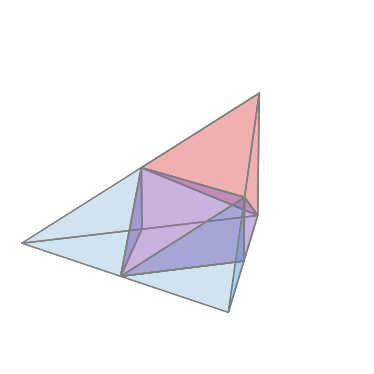
\includegraphics[height=0.5\columnwidth,trim={0.5cm 0.5cm 0.5cm 0.5cm}]{figures/weyl_chamber.pdf}
        \caption{\small Geometric illustration of canonical gates confined to the Weyl chamber.}
        \label{fig:weyl_chamber}
    \end{minipage}
\end{figure}

\footnote{For convenient visualization}


\subsection{Qubit mapping/routing}

Qubit placement and routing ... for connectivity-limited devices


\subsection{Quantum gates realization in diverse ISAs}



\begin{definition}[Canonical gate]
    Any 2Q gate $ U \in \mathbf{SU}(4)$ can be expressed by the composition of its unique \emph{canonical} form
    \begin{align}
        \Can(a,b,c) := e^{-i \frac{\pi}{2}(a\, XX + b\, YY + c\, ZZ)},\, \frac{1}{2} \geq a \geq b \geq \lvert c \rvert
        % U = (A_0\otimes A_1) \Can(a,b,c) (B_0\otimes B_1) = (A_0\otimes A_1) e^{-i \frac{\pi}{2}(a\, XX + b\, YY + c\, ZZ)} (B_0\otimes B_1)
    \end{align}
    sandwiched by local 1Q gates such that we call \emph{$ U $ is locally equivalent to the canonical form $ \Can(a,b,c) $}. %  $ U = (A_0\otimes A_1) \Can(a,b,c) (B_0\otimes B_1) $.
\end{definition}


Canonical representation is ubiquitous as an effective ... 

\ZY{It is ubiquitously used in many quantum computing task ...}




Although there are other conventions .... 
This definition aligns with the \code{TK2} operation definition in \tket, ...



\Cref{fig:weyl_chamber} .....



\begin{align}
    \pSWAP(\theta) \sim \Can(\frac{1}{2},\frac{1}{2},\frac{1}{2}-\frac{\theta}{\pi})
\end{align}



\begin{align}
    \XX(\theta) = \Can(\frac{\theta}{\pi},0,0) \sim \YY(\theta) \sim \ZZ(\theta)
\end{align}

\section{Motivation}\label{sec:motivation}




Two-fold motivations:
\begin{enumerate}
    \item The scalable qubit routing effects (2x-4x) is still a critical challenge in practical quantum computing systems
    \item How to utilize the emerging advanced ISAs (hardware breakthroughs); across all phases of compilation, routing is the bottleneck and is the most easily handled for co-optimization
\end{enumerate}


\ZY{Use a \dquote{optimal routing benchmark} to illustrate the OVERHEAD of existing methods}


\ZY{There should be many takeaways}

\begin{itemize}
    \item Previous routing overhead is not precise for hardware execution
    \item Previous routing is costly and also not precise for hardware execution
    \item SWAP can be implemented in low overhead (gate duration) with the recent breakthrough gate schemes for advanced ISAs 
    \item How to efficiently capture the rich commutation relations when performing co-optimization during qubit routing and gate scheduling
\end{itemize}

\section{\canopus\ framework}\label{sec:canopus}


\subsection{Overview}




\subsection{2Q synthesis cost modeling}\label{sec:2q_synthesis_cost_modeling}



\subsection{Routing in canonical form}\label{sec:routing_in_canonical_form}






- Unified and highly-effective qubit routing approach in canonical form, with properties of quantum ISAs tailored to the routing process


\subsection{Enhanced optimization via commutation}\label{sec:gate_commutation_guided_optimization}

- Capture optimization opportunities exposed by gate commutation; while commutation relations can be uniformly described in canonical form



\begin{theorem}[Canonical gate commutation]\label{thm:commutation}
    Let $\,\Can(a,b,c)_{q_0,q_1}$ and $\,\Can(a',b',c')_{q_1,q_2}$ be two canonical gates acting on qubits ($q_0, q_1$) and ($q_1, q_2$) respectively, with an overlapping qubit $ q_1 $. They are commutative \dquote{if and only if}
    \begin{align}
        b=b'=c=c'=0,
    \end{align}
    that is, when both consist solely of $\,\XX$ rotations.
\end{theorem}






\ZY{Proposition?? Theorem?}




% \subsection{Qubit dependencies guided optimization}\label{sec:qubit_dependencies_guided_optimization}
% - Capture optimization opportunities exposed by qubit dependencies, which implies optimization in a more global scope





\section{Implementation}\label{sec:implementation}



% \documentclass{article}
% \usepackage[ruled,vlined,linesnumbered]{algorithm2e}
% \usepackage{amsmath}

% % Optional: Define a command for code-like text if you prefer a specific style
% \newcommand{\code}[1]{\texttt{#1}}

% \begin{document}

\begin{algorithm}[tbp]
    \caption{Update $L$ when adding a new 2Q gate}
    \label{alg:update_L_D_C}

    \SetKwInOut{KwIn}{Input}
    \SetKwInOut{KwOut}{Output}

    \KwIn{
        $G'$ (Routed DAG), 
        $\pi$ (current logic-to-physical mapping), 
        $L$ (last mapped layer), 
        $D$ (wire durations for each qubit), 
        $C$ (commutative pairs within $L$)
    }
    \KwOut{Updated $G'$, $L$, $D$, $C$}

    \BlankLine

    \tcc{$g$: resolved logical gate;\, $g'$: routed gate}
    $g' \leftarrow G'.\textsc{pushBack}(g, \pi[g.q_0], \pi[g.q_1])$;\, \tcp{$g'.q_i = \pi[g.q_i]$}

    $d \leftarrow \textsc{max}(D[g'.q_0],\, D[g'.q_1]) + \textsc{synthCost}(g)$\;
    $D[g'.q_0] \leftarrow d$; $D[g'.q_1] \leftarrow d$\;

    \For{$\mathrm{pred} \in G'.\textsc{predecessors}(g')$}{
        \If{$\textsc{is2QGate}(\mathrm{pred})$}{
            % \tcp{Distinguish if they are a pair of commutative canonical gates (Theorem 1)}
            \If{$\textsc{isCommutativeCanonicalPair}(g',\, \text{pred})$}{
                $C[(\mathrm{pred}.q_0,\, \text{pred}.q_1)] \leftarrow (g'.q_0,\, g'.q_1)$\;
            }
            \Else{
                $L.\textsc{pop}((\mathrm{pred}.q_0,\, \mathrm{pred}.q_1),\, \textsc{None})$\;
                $C.\textsc{pop}((\mathrm{pred}.q_0,\, \mathrm{pred}.q_1),\, \textsc{None})$\;
            }
        }
        \Else{ 
            \tcc{$ \mathrm{pred\_pred} $ must be None or a 2Q gate}
            $\mathrm{pred\_pred} \leftarrow \textsc{next}(G'.\textsc{predecessors}(\mathrm{pred}))$\;
            \If{$\mathrm{pred\_pred} \neq \textsc{None}$}{
                $L.\textsc{pop}((\mathrm{pred\_pred}.q_0,\, \mathrm{pred\_pred}.q_1),\, \textsc{None})$\;
                $C.\textsc{pop}((\mathrm{pred\_pred}.q_0,\, \mathrm{pred\_pred}.q_1),\, \textsc{None})$\;
            }
        }
    }
    $L[(g'.q_0,\, g'.q_1)] \leftarrow g'$\;

\end{algorithm}

% \end{document}



% \documentclass{article}
% \usepackage[ruled,vlined,linesnumbered]{algorithm2e}
% \usepackage{amsmath} % For \text
% \usepackage{amssymb} % For \Delta

% % Optional: Define a command for code-like text
% \newcommand{\code}[1]{\texttt{#1}}

% \begin{document}

    \begin{algorithm}[tbp]
    \caption{Update $D$ when adding a $ \SWAP $ gate}
    \label{alg:update_durations_swap}

    \SetKwInOut{KwIn}{Input}
    \SetKwInOut{KwOut}{Output}

    \KwIn{
        \code{swap} (encountered SWAP gate), 
        \code{can} (canonical gate within $ L $ on the same qubits as \code{swap}),
        % $D$ (wire durations), 
        % $C$ (commutative pairs within $ L $)
        $ D $, $ C $
    }
    \KwOut{Updated $D$}

    \BlankLine

    % \If{$(\code{swap}.q_0, \code{swap}.q_1) \in C$}{
    %     \tcc{Adjust $ D $ for commutative pair}
    %     $q'_0,\, q'_1 \leftarrow C[(\code{swap}.q_0,\, \code{swap}.q_1)]$\;
    %     \uIf{$\code{swap}.q_0 = q'_0$}{
    %         $D[\code{swap}.q_0] \leftarrow D[q'_0] + \textsc{synthCost}(\text{can})$\;
    %         $D[\code{swap}.q_1] \leftarrow D[\code{swap}.q_0]$\;
    %     }
    %     \ElseIf{$\code{swap}.q_0 = q'_1$}{
    %         $D[\code{swap}.q_0] \leftarrow D[q'_1] + \textsc{synthCost}(\text{can})$\;
    %         $D[\code{swap}.q_1] \leftarrow D[\code{swap}.q_0]$\;
    %     }
    %     \ElseIf{$\code{swap}.q_1 = q'_0$}{
    %         $D[\code{swap}.q_1] \leftarrow D[q'_0] + \textsc{synthCost}(\text{can})$\;
    %         $D[\code{swap}.q_0] \leftarrow D[\code{swap}.q_1]$\;
    %     }
    %     \ElseIf{$\code{swap}.q_1 = q'_1$}{
    %         $D[\code{swap}.q_1] \leftarrow D[q'_1] + \textsc{synthCost}(\text{can})$\;
    %         $D[\code{swap}.q_0] \leftarrow D[\code{swap}.q_1]$\;
    %     }
    % }

    \If{$(\code{swap}.q_0, \code{swap}.q_1) \in C$}{
        % \tcc{Adjust $ D $ for commutative pair}
        $q'_0,\, q'_1 \leftarrow C[(\code{swap}.q_0,\, \code{swap}.q_1)]$\;
        \tcc{Adjust $ D $ by finding matched qubits $q_i \in \{\code{swap}.q_0, \code{swap}.q_1\}$ and $q'_j \in \{q'_0, q'_1\}$}
        $D[q_i] \leftarrow D[q'_j] + \textsc{synthCost}(\text{can})$\;
        $D[\text{the other \code{swap} qubit}] \leftarrow D[q_i]$\;
    }
    % \BlankLine

    % \tcc{Calculate circuit depth increment}
    % $\Delta_{\text{depth}} \leftarrow \textsc{synthCost}(\code{can}.\textsc{mirror}()) - \textsc{synthCost}(\text{can})$\;
    $d \leftarrow \textsc{max}(D[\code{swap}.q_0],\, D[\code{swap}.q_1]) + \textsc{synthCost}(\code{can}.\textsc{mirror}()) - \textsc{synthCost}(\text{can})$\;
    $D[\code{swap}.q_0] \leftarrow d$; $D[\code{swap}.q_1] \leftarrow d$\;

\end{algorithm}

% \end{document}



\subsection{Core functionalities}


\subsection{Extensions}



\subsection{Scalability}\label{sec:scalability}

\section{Case Studies}\label{sec:studies}

\subsection{QFT kernel}

\subsection{Co-exploration of routing and ISA selection}
% TODO: 什么样的电路pattern适合什么样的ISA(以及ISA实现方式)?



\subsection{Stabilizer circuit}



\subsection{Mapping on FTQC architecture}
% TODO: 比如QFT电路

\section{Evaluation}\label{sec:evaluation}



\begin{table}[tbp]
    \centering
    \caption{Benchmarks information. These metrics are collected from the circuits after logical-level optimization by \tket, thus including only $\Can$ and $\Uthree$ gates. Circuit cost (Duration $T$) is calculated in \CXISA ISA.}
    
    \label{tab:benchmark}
    % \setlength{\tabcolsep}{2.5pt}
    % \fontsize{4.6}{5.0}\selectfont
    \begin{small}
        \begin{tabular}{|l|r|r|r|r|}
\toprule
Program & #Qubit & #Can & Depth2Q & Cost \\
\midrule
bigadder & 18 & 114 & 79 & 88.0 \\
bv & 19 & 18 & 18 & 18.0 \\
gcm & 13 & 377 & 376 & 510.0 \\
ising & 26 & 25 & 2 & 4.0 \\
knn & 25 & 72 & 50 & 62.0 \\
multiplier & 15 & 198 & 122 & 133.0 \\
qec9xz & 17 & 32 & 12 & 12.0 \\
qft & 18 & 153 & 33 & 66.0 \\
qpeexact & 16 & 127 & 43 & 86.0 \\
qram & 20 & 110 & 70 & 78.0 \\
sat & 11 & 210 & 182 & 204.0 \\
swap & 25 & 72 & 50 & 62.0 \\
wstate & 27 & 52 & 28 & 28.0 \\
\bottomrule
\end{tabular}

    \end{small}

\end{table}




\begin{figure*}[t]
    
    \centering
    \includegraphics[width=\textwidth]{figures/detailed_results.pdf}

    \caption{Detailed benchmarking results for different compilers (\sabre, \toqm, \bqskit, \canopus) across diverse topologies (columns from left to right: 1D Chain, 2D HHex, 2D Square) and quantum ISAs (rows from top to bottom: \CXISA, \ZZPhaseISA, \SQiSWISA, \ZZPhaseWithMirrorISA, \SQiSWWithMirrorISA, \HetISA). Sizes and colors of the bubbles represent the values for routing overhead (multiples of the routed and rebased circuits compared to that of prior-routing ones).}
    \label{fig:detailed_results}
    
\end{figure*}



\begin{table*}[tbp]
    \centering
    \caption{Summarized results for the routing overhead with average (geometric-mean) values emphasized.}
    \label{tab:summarized_results}

    % \setlength{\tabcolsep}{2.5pt}
    % \begin{scriptsize}
    % \begin{small}
        % \begin{tabular}{|l|r|r|r|r|r|r|r|r|}
% \hline
% &
% \multicolumn{4}{c|}{\textbf{Routing overhead (\CXISA)}} &
% \multicolumn{4}{c|}{\textbf{Routing overhead (\ZZPhaseISA)}} &
% \multicolumn{4}{c|}{\textbf{Routing overhead (\SQiSWISA)}} &
% \multicolumn{4}{c|}{\textbf{Routing overhead (\ZZPhaseWithMirrorISA)}} &
% \multicolumn{4}{c|}{\textbf{Routing overhead (\SQiSWWithMirrorISA)}} &
% \multicolumn{4}{c|}{\textbf{Routing overhead (\HetISA)}} \\
% \hline
% Topology & \sabre & \toqm & \bqskit & \canopus & \sabre & \toqm & \bqskit & \canopus & \sabre & \toqm & \bqskit & \canopus & \sabre & \toqm & \bqskit & \canopus & \sabre & \toqm & \bqskit & \canopus & \sabre & \toqm & \bqskit & \canopus \\
% \hline
% Chain & 2.94 & 2.67 & 2.33 & 1.84 & 2.66 & 2.52 & 2.11 & 1.64 & 2.58 & 2.26 & 1.97 & 1.66 & 2.10 & 1.94 & 1.81 & 1.33 & 2.18 & 1.93 & 1.76 & 1.44 & 2.15 & 2.00 & 1.69 & 1.32 \\
% \hline
% HHex & 2.93 & 2.56 & 2.65 & 1.85 & 2.63 & 2.37 & 2.29 & 1.70 & 2.61 & 2.33 & 2.29 & 1.69 & 2.09 & 1.90 & 1.97 & 1.34 & 2.20 & 1.94 & 2.12 & 1.48 & 2.15 & 1.94 & 1.97 & 1.39 \\
% \hline
% Square & 2.18 & 2.02 & 2.42 & 1.44 & 1.89 & 1.79 & 1.92 & 1.21 & 2.08 & 1.91 & 1.99 & 1.42 & 1.57 & 1.47 & 1.66 & 1.01 & 1.70 & 1.56 & 1.79 & 1.18 & 1.60 & 1.50 & 1.57 & 1.04 \\
% \hline
% \end{tabular}




\begin{tabular}{|l|r|r|r|r|r|r|r|r|}
\hline
 & \multicolumn{4}{c|}{\textbf{Routing overhead (\CXISA)}} & \multicolumn{4}{c|}{\textbf{Routing overhead (\ZZPhaseISA)}} \\
\hline
\textbf{Topology} & \sabre & \toqm & \bqskit & \canopus & \sabre & \toqm & \bqskit & \canopus \\
\hline
Chain & 2.93x & 2.67x & 2.34x & \textbf{1.73}x & 2.63x & 2.51x & 2.17x & \textbf{1.61}x \\
\hline
HHex & 2.90x & 2.56x & 2.66x & \textbf{1.81}x & 2.62x & 2.37x & 2.26x & \textbf{1.70}x \\
\hline
Square & 2.14x & 2.04x & 2.47x & \textbf{1.42}x & 1.87x & 1.82x & 1.94x & \textbf{1.19}x \\
% \hline
% \end{tabular}

% \begin{tabular}{|l|r|r|r|r|r|r|r|r|}
\hline
 & \multicolumn{4}{c|}{\textbf{Routing overhead (\SQiSWISA)}} & \multicolumn{4}{c|}{\textbf{Routing overhead (\ZZPhaseWithMirrorISA)}} \\
\hline
\textbf{Topology} & \sabre & \toqm & \bqskit & \canopus & \sabre & \toqm & \bqskit & \canopus \\
\hline
Chain & 2.57x & 2.27x & 2.00x & \textbf{1.55}x & 2.08x & 1.94x & 1.87x & \textbf{1.26}x \\
\hline
HHex & 2.59x & 2.33x & 2.28x & \textbf{1.65}x & 2.08x & 1.90x & 1.96x & \textbf{1.33}x \\
\hline
Square & 2.05x & 1.94x & 2.02x & \textbf{1.39}x & 1.54x & 1.49x & 1.65x & \textbf{1.00}x \\
% \hline
% \end{tabular}

% \begin{tabular}{|l|r|r|r|r|r|r|r|r|}
\hline
 & \multicolumn{4}{c|}{\textbf{Routing overhead (\SQiSWWithMirrorISA)}} & \multicolumn{4}{c|}{\textbf{Routing overhead (\HetISA)}} \\
\hline
\textbf{Topology} & \sabre & \toqm & \bqskit & \canopus & \sabre & \toqm & \bqskit & \canopus \\
\hline
Chain & 2.17x & 1.93x & 1.78x & \textbf{1.38}x & 2.13x & 2.00x & 1.74x & \textbf{1.29}x \\
\hline
HHex & 2.17x & 1.93x & 2.10x & \textbf{1.42}x & 2.13x & 1.94x & 1.98x & \textbf{1.37}x \\
\hline
Square & 1.67x & 1.58x & 1.83x & \textbf{1.15}x & 1.58x & 1.52x & 1.56x & \textbf{1.02}x \\
\hline
\end{tabular}

    % \end{scriptsize}
    % \end{small}

\end{table*}

\section{Related Works}\label{sec:related}

Qubit mapping/routing is one the the most well-explored topic of quantum compiler research, as it shares the similar methodologies with instruction scheduling~\cite{codina2001unified,hennessy1983postpass} and register allocation~\cite{chaitin1982register,poletto1999linear} in classical computing. Conventional methods focus on the simplified routing model, that is, \#$ \SWAP $-minimal insertion, three-$ \CX $-unrolled $ \SWAP $ gate, and $ \CX $-based latency metric. That brings a gap between quantum hardware performance and its ceiling, which is particularly evident with the progress of underlying instruction models for modern quantum hardware.


\citet{zulehner2018efficient} introduces an A*-based algorithm to minimize SWAP gate overhead for concurrent CNOT gate layers. The approach partitions the circuit into layers and solves the mapping problem subsequently. \citet{li2019tackling} also utilizes the circuit DAG layering thought to tackle the qubit mapping problem and proposes the bidirectional routing procedure to acquire a better initial mapping desired to result in \#$ \SWAP $ inserted minimization as expected. It also briefly discusses the trade-off between the inserted $ \SWAP $ count and the circuit depth but does not prioritize optimizing circuit depth. Some other works leverage algorithmic procedures similar to \sabre\ to improve parallelism among inserted $\SWAP$s and other 2Q gates~\cite{lao2021timing,ddroute2025,zou2024lightsabre}, or attempt to minimize circuit depth via graph matching~\cite{childs2019circuit}. \citet{zhang2021time} systematically investigates the time (circuit depth) optimality of qubit mapping and proposed an A*-based method \toqm\ that results in better results than the SOTA solver-based depth-driven algorithm~\cite{tan2020optimal}. However, the optimality of qubit routing is a complex task. There are rarely theoretical studies that claims the holistic optimality of some $ \SWAP $ insertion schemes provided the quantum ISAs, device topologies, and synthesis cost models. In our field tests, TOQM does not lead to time-optimal results compared to our heuristic \canopus, and the optimal mapping scheme for specific patterns such as QFT kernel analyzed in \cite{zhang2021time} are not indeed optimal, according to our case study in \Cref{sec:qft_study}.

With the recent development of advanced quantum ISAs such as superconducting fractional gates~\cite{ibmFractionalGates}, ion-trapped partial entangling gates~\cite{ionqPartialGates,yale2025realization}, and the AshN scheme~\cite{chen2024one}, some works began exploring how to efficiently utilize these ISAs to make compiler optimizations closer to hardware characteristics. \citet{mckinney2024mirage} investigates the practical performance of \SQiSWISA\ ISA proposed by \citet{huang2023quantum} and the synthesis capability when incorporating the basis gates' mirrors into the ISA. The modified \sabre\ algorithm in \cite{mckinney2024mirage} provides an attempt of the collaborative gate decomposition and qubit routing approach, while the optimization opportunities considered therein are limited and the algorithmic techniques are not sophisticated. \bqskit~\cite{bqskit} and the series of works behind~\cite{davis2019heuristics,wu2020qgo,kukliansky2023qfactor,younis2021qfast} provides a toolkit to rebase arbitrary 2Q unitaries to specific ISAs through approximate synthesis (structural search and numerical optimization) that is not computational efficient. Approximate synthesis by \bqskit does not ensure an optimal schemes for two-qubit and multi-qubit synthesis cases. In addition, due to the lack of native compilation strategies and rational synthesis cost model, \citet{kalloor2024quantum} claims that alternative ISAs are hard to be comparable to \CXISA\ when evaluating quantum hardware roofline by \bqskit. As for applicability of expanded ISAs to QEC, Google's latest theoretical~\cite{mcewen2023relaxing} and experimental~\cite{eickbusch2024demonstrating} works demonstrate the \CXISA-\iSWAPISA\ combination ISA could benefits suppressing fault-tolerant threshold. \citet{zhou2024halma} proposes a routing-based method enhanced by \CXISA-\iSWAPISA\ for overcoming ancilla defects among surface code blocks while preserving encoded logical information.



% - expanded ISAs \& systematic utilization
%     - Noise-aware ...
%     - Mirage ... not sophisticated algorithm, ... a subset of our approach
%     - BQSKit ... quantum hardware roofline .. they claim that ... 
%     - The last-step \dquote{synthesizer} .... most based on \dquote{approximate synthesis} (roofline, heterogeneous, ZZ(theta))

% (((((((None of them make deep co-optimization tailored to various quantum ISAs in a systematic and efficient approach)))))))


% With respect to the heuristic cost for $ \SWAP $ search, our routing algorithm involves the duration (generalization metric of circuit depth) driven goal by taking the canonical gate synthesis cost into the circuit duration increment. 




\section{Conclusion}\label{sec:conclusion}




It is promising to explore novel Clifford circuit optimization techniques drawing on the canonical gate representation.







% use the ACM bibliography style
\bibliographystyle{ACM-Reference-Format}
\bibliography{reference}


%%%%%%----- Appendix -----%%%%%%
\onecolumn
\appendix
\section{Canonical gate and 2Q circuit synthesis}\label{sec:appendix_A}


In this section we show the basic mathematical properties the its canonical form of 2Q unitary and then discuss the synthesis capability of some 2Q basis gates.

\subsection{Canonical decomposition}

$\mathbf{SU}(N)$ is a real manifold with dimension $N^2 - 1$, within which any element is a \emph{special unitary} matrix with determinant equal to 1. Since the global phase does not affect quantum computation processes, it is sufficient to focus on the mathematical properties of special unitaries in the area of circuit synthesis. A generic 2Q gate, despite having 15 real parameters, can have its nonlocal behavior fully characterized by only 3 real parameters. This method, known as \emph{Canonical decomposition} or \emph{KAK decomposition} from Lie algebra theory, is widely adopted in quantum computing~\cite{zhang2003geometric,tucci2005introduction,bullock2003arbitrary,zulehner2019compiling}. Specifically, for any $U \in \mathbf{SU}(4)$, there exists a unique $\vec{\eta} = (x, y, z) \in W \subseteq \mathbb{R}^3$, along with $V_1, V_2, V_3, V_4 \in \mathbf{SU}(2)$ and a global phase, such that
\begin{align}
U = g \cdot (V_1 \otimes V_2) e^{-i\vec{\eta} \cdot \vec{\Sigma}} (V_3 \otimes V_4),\, g \in \{1, i\}
\end{align}
where $\vec{\Sigma} \equiv (XX, YY, ZZ)$~\cite{tucci2005introduction}. The set
\begin{align}
W := \left\{(x, y, z) \in \mathbb{R}^3 \,\vert\, \frac{\pi}{4} \geq x \geq y \geq |z|,\, z \geq 0 \text{ if } x = \frac{\pi}{4}\right\}
\end{align}
is known as the \emph{Weyl chamber}~\cite{zhang2003geometric}, and  $\vec{\eta} \in W$ is known as the \emph{Weyl coordinate} of $ U $. We also refer to a gate of the form 
\begin{align}
    \Can(a,b,c):= e^{-i\frac{\pi}{2}(a\,XX+b\,YY+c\,ZZ)} = \begin{pmatrix}
        e^{-i \frac{c\pi}{2}} \cos{\frac{(a-b)\pi}{2}} & 0 & 0 & -i e^{-i \frac{c\pi}{2}} \sin{\frac{(a-b)\pi}{2}} \\
        0 & e^{i \frac{c\pi}{2}} \cos{\frac{(a+b)\pi}{2}} & -i e^{i \frac{c\pi}{2}} \sin{\frac{(a+b)\pi}{2}} & 0 \\
        0 & -i e^{i \frac{c\pi}{2}} \sin{\frac{(a+b)\pi}{2}} & e^{i \frac{c\pi}{2}} \cos{\frac{(a+b)\pi}{2}} & 0 \\
        -i e^{-i \frac{c\pi}{2}} \sin{\frac{(a-b)\pi}{2}} & 0 & 0 & e^{-i \frac{c\pi}{2}} \cos{\frac{(a-b)\pi}{2}}
    \end{pmatrix}
\end{align}
as a \emph{canonical} gate. Two 2Q gates $ U $ and $ V $ are considered \emph{locally equivalent} if they differ only by 1Q gates, meaning their canonical coefficients can be transformed into one another via the equivalence rules~\cite{crooks2020gates}:
\begin{enumerate}
    \item $(a,b,c)\sim (b,a,c)$ or $(a,b,c)\sim (c,b,a)$, i.e., any permutation of the coefficients;
    \item $(a,b,c)\sim (-a, -b, c)$;
    \item $(a,b,c)\sim (a-1, b, c)$;
    \item $(1/2, b, c) \sim (1/2, b, -c)$.
\end{enumerate}
Note that we align the conventional that canonical coefficient $ (a,b,c) $ differs from Weyl coordinate $ (x,y,z) $ by a $ \frac{\pi}{2} $ factor. Unless otherwise specified, the canonical coefficients of gates in quantum ISAs and circuits are confined to $ \frac{1}{2}\geq a \geq b \geq \lvert c\rvert $. While for the Weyl chamber visualization by means of \code{weylchamber}, we assume the Weyl coordinates are confined to $\left\{\frac{\pi}{4}\geq x \geq y \geq z\geq 0\right\} \cup \left\{\frac{\pi}{4} \geq \frac{\pi}{2}-x \geq y \geq z \geq 0\right\}$, as illustrated by \Cref{fig:weyl_chamber}. Conversion of Weyl coordinates for different conventions is not simple according to the equivalence rules above.






\subsection{Quantum ISA and the synthesis capability}




\subsection{2Q gate mirroring}

% TODO: 


Mirroring formula:



% \begin{align}
%     \mathrm{SWAP}\cdot\mathrm{Can}(a,b,c)
%     \sim \left(x+\frac{1}{2}, y+\frac{1}{2}, z+\frac{1}{2}\right)
%     \sim \left(x+\frac{1}{2}-1,y+\frac{1}{2}-1,z+\frac{1}{2}-1\right)
%     \sim  \left\{
%     \begin{cases}{ll}
%     \left(\frac{1}{2}-z, \frac{1}{2}-y, x - \frac{1}{2}\right), \textrm{ if } z\geq 0 \\
%     \left(\frac{1}{2} + z, \frac{1}{2}-y, \frac{1}{2} - x\right), \textrm{ if } z < 0
%     \end{cases}
%     \right.
% \end{align}

\begin{align}
    \mathrm{SWAP} \cdot \mathrm{Can}(a,b,c)
    & \sim \left(x+\frac{1}{2}, y+\frac{1}{2}, z+\frac{1}{2}\right) 
    & \sim \left(x+\frac{1}{2}-1, y+\frac{1}{2}-1, z+\frac{1}{2}-1\right) 
    & \sim
    \begin{cases}
        \left(\frac{1}{2}-z, \frac{1}{2}-y, x - \frac{1}{2}\right), & \text{if } z \geq 0 \\
        \left(\frac{1}{2} + z, \frac{1}{2}-y, \frac{1}{2} - x\right), & \text{if } z < 0
    \end{cases}
\end{align}


\subsection{Coverage sets for the selected ISAs used in ...}




\begin{figure}[tbp]
    \centering
    \begin{minipage}[t]{0.48\textwidth}
        \centering
        \includegraphics[width=\textwidth]{figures/coverage/coverage_cx_minimal.pdf}
        \caption{Coverage set for \CXISA\ ISA.}
        \label{fig:coverage_cx}
    \end{minipage}
    \hfill
    \begin{minipage}[t]{0.48\textwidth}
        \centering
        \includegraphics[width=\textwidth]{figures/coverage/coverage_sqisw_minimal.pdf}
        \caption{Coverage set for \SQiSWISA\ ISA.}
        \label{fig:coverage_sqisw}
    \end{minipage}
\end{figure}



\begin{figure}[tbp]
    \centering
    \includegraphics[width=\textwidth]{figures/coverage/coverage_sqisw_with_mirror_minimal.pdf}
    \caption{Coverage set for \SQiSWWithMirrorISA\ ISA.}
    \label{fig:coverage_sqisw_with_mirror}
\end{figure}




\begin{figure}[tbp]
    \centering
    \includegraphics[width=\textwidth]{figures/coverage/coverage_zzphase_minimal_1.pdf}\vspace{-1.5em}
    \includegraphics[width=\textwidth]{figures/coverage/coverage_zzphase_minimal_2.pdf}\vspace{-1.5em}
    \includegraphics[width=0.83\textwidth]{figures/coverage/coverage_zzphase_minimal_3.pdf}\vspace{-2em}
    \caption{Coverage set for \ZZPhaseISA\ ISA.}
    \label{fig:coverage_zzphase}
\end{figure}



\begin{figure}[tbp]
    \centering
    \includegraphics[width=\textwidth]{figures/coverage/coverage_zzphase_with_mirror_minimal_1.pdf}\vspace{-1.5em}
    \includegraphics[width=\textwidth]{figures/coverage/coverage_zzphase_with_mirror_minimal_2.pdf}\vspace{-1.5em}
    \includegraphics[width=\textwidth]{figures/coverage/coverage_zzphase_with_mirror_minimal_3.pdf}\vspace{-1.5em}
    \includegraphics[width=0.5\textwidth]{figures/coverage/coverage_zzphase_with_mirror_minimal_4.pdf}\vspace{-2em}
    \caption{Coverage set for \ZZPhaseWithMirrorISA\ ISA.}
    \label{fig:coverage_zzphase_with_mirror}
\end{figure}




\begin{figure}[tbp]
    \centering
    \includegraphics[width=\textwidth]{figures/coverage/coverage_het_minimal_1.pdf}\vspace{-1.5em}
    \includegraphics[width=\textwidth]{figures/coverage/coverage_het_minimal_2.pdf}\vspace{-1.5em}
    \includegraphics[width=\textwidth]{figures/coverage/coverage_het_minimal_3.pdf}\vspace{-1.5em}
    \includegraphics[width=0.66\textwidth]{figures/coverage/coverage_het_minimal_4.pdf}\vspace{-2em}
    \caption{Coverage set for \HetISA\ ISA.}
    \label{fig:coverage_het}
\end{figure}







\section{Commutative relation of canonical gates}\label{sec:appendix_B}

Herein we present detailed proof for \Cref{thm:commutation}. The \textit{if} direction is trivial, and hence we justify the \textit{only if} direction, relying on the following two lemmas.

\begin{lemma}\label{lemma:hamiltonian_exponential}
Let $A$, $B$ be two Hermitian matrices with eigenvalues in the range $[-2,2)$. If $[e^{-i\frac{\pi}{2}A},e^{-i\frac{\pi}{2}B}]=0$ then $[A,B]=0$.
\end{lemma}
\begin{proof}
This follows from the fact that compatible observables (commuting operators) can be simultaneously diagonalized. In this case, the respective unitary matrix $e^{-i\frac{\pi}{2}A}$ commutes with $e^{-i\frac{\pi}{2}B}$. Denote by $A_{\lambda}$ the eigenspace corresponding to the eigenvalue $\lambda$ of $e^{-i\frac{\pi}{2}A}$, i.e. $e^{-i\frac{\pi}{2}A} = \oplus_{\lambda} \lambda A_{\lambda}$. Then we have
\begin{align}
    \forall \vec{v} \in A_\lambda,\, e^{-i\frac{\pi}{2}B}e^{-i\frac{\pi}{2}A}\vec{v}=e^{-i\frac{\pi}{2}B}\lambda \vec{v}=\lambda e^{-i\frac{\pi}{2}B}\vec{v}=e^{-i\frac{\pi}{2}A}e^{-i\frac{\pi}{2}B}\vec{v},
\end{align}

and thus $e^{-i\frac{\pi}{2}B}\vec{v}\in A_\lambda$. Thus $A_\lambda$ is $e^{-i\frac{\pi}{2}B}$-invariant and the restriction $e^{-i\frac{\pi}{2}B}\big\rvert_{A_{\lambda}}$ of $e^{-i\frac{\pi}{2}B}$ to $A_{\lambda}$ is still unitary since it preserves inner products. Hence it is diagonalizable and we can find an orthonormal basis $w_{\lambda_1},w_{\lambda_2},\ldots,w_{\lambda_k}$ consisting of eigenvectors of $e^{-i\frac{\pi}{2}B}\big\rvert_{A_{\lambda}}$. Note that these are also eigenvectors of $e^{-i\frac{\pi}{2}A}$ (with eigenvalue $\lambda$). Following the same token as above, for each eigenspace $E_{\lambda_i}$ of $e^{-i\frac{\pi}{2}A}$, we can construct an orthonormal basis $\beta_i$ for it consisting of eigenvectors of $e^{-i\frac{\pi}{2}B}$. Finally since the eigenspaces of different eigenvalues of $e^{-i\frac{\pi}{2}A}$ are orthogonal to each other, $\beta=\cup_i\beta_i$ forms an orthonormal basis of the entire Hilbert space $\mathcal{H}_n$ consisting of the coeigenvectors of both $e^{-i\frac{\pi}{2}A}$ and $e^{-i\frac{\pi}{2}B}$.

Now let $U$ be a unitary matrix with the vectors in $\beta$ being its columns, then
\begin{align}
    \begin{aligned}
    U^\dagger e^{-i\frac{\pi}{2}A}U&=D_A\\
    U^\dagger e^{-i\frac{\pi}{2}B}U&=D_B
    \end{aligned}
\end{align}

In general, an eigenvector of $e^{-i\frac{\pi}{2}A}$ need \textit{not} be that of $A$. However, since $A$ has its eigenvalues in the range $[-2,2)$, the map
\begin{align}
    f:[-2,2)\rightarrow U(1),a\rightarrow e^{-i\frac{\pi}{2}a}
\end{align}
is injective. Consequently different eigenvalues of $A$ correspond to different eigenvalues of $e^{-i\frac{\pi}{2}A}$, and hence the eigenspaces of $e^{-i\frac{\pi}{2}A}$ and $A$ coincide. Therefore, we have that
\begin{align}
    \begin{aligned}
    U^\dagger AU&=\Sigma_A\\
    U^\dagger BU&=\Sigma_B
    \end{aligned}
\end{align}
and since $[\Sigma_A,\Sigma_B]=0$ as they are diagonal, $[A,B]=0$. We obtain the desired result.

\end{proof}


\begin{lemma}\label{lemma:xx_rotation}
Let $P_1=(a_1X_1X_2+b_1Y_1Y_2+c_1Z_1Z_2)I_3$, $P_2=I_1(a_2X_2X_3+b_2Y_2Y_3+c_2Z_2Z_3)$ with $|c_1|\le b_1\le a_1\le\frac{1}{2}$, $|c_2|\le b_2\le a_2\le\frac{1}{2}$. If $[P_1,P_2]=0$ and $P_1,P_2\ne0$, then $b_1=b_2=c_1=c_2=0$.
\end{lemma}
\begin{proof}
Consider the product $P_1P_2$. We assume for the sake of contradiction that $b_1\ne0$. Using $[X,Y]=2iZ$, $[Y,Z]=2iX$, $[Z,X]=2iY$, we expand
\begin{align*}
[P_1,P_2] &= 2i\bigl(a_1b_2\,X_1Z_2Y_3 - b_1a_2\,Y_1Z_2X_3 + b_1c_2\,Y_1X_2Z_3\bigr) -2i\bigl(a_1c_2\,X_1Y_2Z_3 + c_1a_2\,Z_1Y_2X_3 + c_1b_2\,Z_1X_2Y_3\bigr).
\end{align*}
Since the each Pauli string is linearly independent in the $8\times8$ operator basis, e.g. term $Y_1Z_2X_3$ cannot be canceled out by any other terms, contradictory to the fact that $[P_1,P_2]=0$. Hence, vanishing of $[P_1,P_2]$ requires
\begin{align*}
a_1b_2 = a_1c_2 = b_1c_2 = b_1a_2 = c_1a_2 = c_1b_2 = 0.
\end{align*}
Since $P_1,P_2\neq0$, at least $a_1,a_2$ is nonzero, leading to $b_1 = b_2=c_1=c_2=0$. 
\end{proof}

Using \Cref{lemma:hamiltonian_exponential} and \Cref{lemma:xx_rotation} above, it is straightforward to prove \Cref{thm:commutation}. We see that $\|P_1\|\le\|a_1X_1X_2I_3\|+\|b_1Y_1Y_2I_3\|+\|c_1Z_1Z_2I_3\|\le|a_1|+|b_1|+|c_1|\le\frac{3}{2}$, where $\|\cdot\|$ is the operator norm. Hence, eigenvalues of $P_1$ are in range of $[-2,2)$. Same as the eigenvalues of $P_2$. Now if $[e^{-i\frac{\pi}{2}P_1},e^{-i\frac{\pi}{2}P_2}]=0$, then we have that $[P_1,P_2]=0$ according to \Cref{lemma:hamiltonian_exponential}, and thus $b_1=b_2=c_1=c_2=0$ according to \Cref{lemma:xx_rotation}, which proves the \textit{only if} direction.


\section{Commutation relation between canonical gates}\label{sec:appendix_C}

Herein we present detailed proof for \Cref{thm:commutation}, relying on the following two lemmas.




\end{document}
